% Constraints on Higgs-charm couplings at CMS
% Higgs 2026, Louvain-la-Neuve, 28 Oct 2026 (15+5 min)
% v2: Moloch theme + ICNFP-style boxes, pills and callout arrows (hccstyle.sty).
% Every number and figure below is from a public CMS paper / PAS / DP note.
% Figures: re-download with fetch_figures.sh. Build: latexmk -pdf higgs2026_higgs_charm_v2.tex
\documentclass[aspectratio=169,10pt,xcolor=table]{beamer}
\usetheme{moloch}
\usefonttheme{professionalfonts}
\usepackage[T1]{fontenc}
\usepackage[sfdefault]{FiraSans}
\usepackage{newtxsf}
\definecolor{accA}{HTML}{23373B}   % boxes, pills
\definecolor{accB}{HTML}{EB811B}   % callouts, results
\colorlet{cmsblue}{accA}
\colorlet{cmsorange}{accB}
\colorlet{cmsgrey}{gray}
\colorlet{cmslight}{accA!9}
\usepackage{hccstyle}
\usepackage{amsmath,amssymb,booktabs,array,graphicx}
\usepackage{hyperref}
\hypersetup{colorlinks=false,pdfborder={0 0 0}}
% upright math letters (H, c, Z, ...) in the sans font
\DeclareSymbolFont{operators}{\encodingdefault}{\sfdefault}{m}{n}
\SetSymbolFont{operators}{bold}{\encodingdefault}{\sfdefault}{b}{n}
\DeclareMathAlphabet{\mathrm}{\encodingdefault}{\sfdefault}{m}{n}
\SetMathAlphabet{\mathrm}{bold}{\encodingdefault}{\sfdefault}{b}{n}
\tikzset{
  fermion/.style={thick,accA,postaction={decorate},decoration={markings,mark=at position 0.55 with {\arrow{Stealth}}}},
  antifermion/.style={thick,accA,postaction={decorate},decoration={markings,mark=at position 0.55 with {\arrow{Stealth[reversed]}}}},
  higgs/.style={thick,dashed,accA},
  gluon/.style={thick,accA,decorate,decoration={coil,amplitude=2.2pt,segment length=3.6pt}},
  kcvertex/.style={circle,fill=accB,inner sep=1.8pt}}
\graphicspath{{figures/}}

\newcommand{\qbar}[1]{\mathrm{#1}\overline{\mathrm{#1}}}
\newcommand{\ccbar}{\ensuremath{\qbar{c}}}
\newcommand{\bbbar}{\ensuremath{\qbar{b}}}
\newcommand{\kc}{\ensuremath{\kappa_\mathrm{c}}}
\newcommand{\kb}{\ensuremath{\kappa_\mathrm{b}}}
\newcommand{\Hcc}{\ensuremath{\mathrm{H}\to\qbar{c}}}
\newcommand{\Hbb}{\ensuremath{\mathrm{H}\to\qbar{b}}}
\newcommand{\ttH}{\ensuremath{\qbar{t}\mathrm{H}}}
\newcommand{\ttbar}{\ensuremath{\qbar{t}}}
\newcommand{\ttZ}{\ensuremath{\qbar{t}\mathrm{Z}}}
\newcommand{\fbinv}{\ensuremath{\,\mathrm{fb}^{-1}}}
\newcommand{\new}{{\color{accB}\textbf{\scriptsize NEW}}}
\newcommand{\obsexp}[2]{#1\,{\color{gray}(#2)}}
\newcommand{\tobackup}{{\scriptsize\color{gray}$\to$ backup}}
\newcommand{\pubHIG}[1]{https://cms-results.web.cern.ch/cms-results/public-results/publications/#1/}
% take-away line: orange arrow + italic message
\newcommand{\takeaway}[1]{\par\vspace{2pt}{\centering\tikz[baseline=-0.6ex]\draw[callout] (0,0) -- (0.5,0);\ \callnote{\normalsize #1}\par}}
% paper reference, printed in the title bar; call \pubref{...} right before \begin{frame}
\newcommand{\pubref}[1]{\gdef\thepubref{#1}}
\gdef\thepubref{}
\addtobeamertemplate{frametitle}{}{\begin{tikzpicture}[remember picture,overlay]
  \node[anchor=north east,font=\scriptsize,text=gray!70] at ([xshift=-3mm,yshift=-1.2mm]current page.north east) {\thepubref};\end{tikzpicture}\gdef\thepubref{}}
\newcommand{\up}{\vspace*{-0.8em}}
\newcommand{\rref}[1]{\hfill{\scriptsize\color{gray}#1}}

\title{Constraints on Higgs-charm couplings at CMS}
\author{Chirayu Gupta\\{\small on behalf of the CMS Collaboration}}
\institute{Vrije Universiteit Brussel}
\date{Higgs 2026, Louvain-la-Neuve, 28 October 2026}
\titlegraphic{\includegraphics[height=1.0cm]{CMSlogo_color.png}\hspace{0.4cm}\includegraphics[height=1.0cm]{VUB_logo.png}}

\begin{document}

% ===================================================================
\begin{frame}[plain]
  \titlepage
  \begin{tikzpicture}[remember picture,overlay]
    % production (gc -> cH) and decay (H -> cc): kc at the orange vertices
    \begin{scope}[shift={([xshift=-5.6cm,yshift=1.7cm]current page.south east)},font=\small]
      \draw[gluon] (0,0.7) node[left,accA]{g} -- (0.8,0);
      \draw[fermion] (0,-0.7) node[left,accA]{c} -- (0.8,0);
      \draw[fermion] (0.8,0) -- (1.6,0);
      \draw[fermion] (1.6,0) -- (2.4,0.7) node[right,accA]{c};
      \draw[higgs] (1.6,0) -- (2.4,-0.7) node[right,accA]{H};
      \node[kcvertex] at (1.6,0) {};
      \node[accB,below=2pt] at (1.6,-0.05) {$\kappa_\mathrm{c}$};
    \end{scope}
    \begin{scope}[shift={([xshift=-2.4cm,yshift=1.7cm]current page.south east)},font=\small]
      \draw[higgs] (0,0) node[left,accA]{H} -- (1.0,0);
      \draw[fermion] (1.0,0) -- (1.7,0.7) node[right,accA]{c};
      \draw[antifermion] (1.0,0) -- (1.7,-0.7) node[right,accA]{$\overline{\mathrm{c}}$};
      \node[kcvertex] at (1.0,0) {};
      \node[accB,left=3pt] at (1.0,-0.35) {$\kappa_\mathrm{c}$};
    \end{scope}
  \end{tikzpicture}
\end{frame}

% ===================================================================
\begin{frame}[t]{Why the Higgs-charm coupling?}
  \up
  \begin{columns}[T]
    \column{0.585\textwidth}
    \pill{Yukawa couplings today}\par\vspace{2pt}
    {\small Since 2012: couplings to t, b, $\tau$ measured; evidence for H$\to\mu\mu$ \tobackup; all SM-like\par}
    \vspace{3pt}
    \pill{Why charm?}\par\vspace{2pt}
    \begin{keybox}
      \textbf{2\textsuperscript{nd}-generation quark Yukawas are the open frontier}; charm is the most accessible\\[2pt]
      $\bullet$ $\mathcal{B}(\Hcc)\approx 2.9\%$, about 20$\times$ below \Hbb\\
      $\bullet$ huge QCD backgrounds; c jets are hard to tell from b and light jets (slide 4)
    \end{keybox}
    {\centering $\kc = y_\mathrm{c}/y_\mathrm{c}^\mathrm{SM}$\quad{\small (SM: $\kc=1$)}\par}
    \vspace{2pt}
    \begin{resultbox}[fontupper=\footnotesize]
      Flavour-compatible BSM (e.g.\ spontaneous flavour violation) allows $|\kc|\sim3$:\\
      \textbf{current sensitivity is entering this region}
    \end{resultbox}
    \takeaway{Does the Higgs give charm its mass?}

    \column{0.395\textwidth}
    \centering
    \includegraphics[height=5.4cm]{HIG-21-018_Figure-aux_011.pdf}\\
    {\scriptsize CMS, Rep.\ Prog.\ Phys.\ 89 (2026) 087801 (suppl.); \kc\ point: separate \ttH+VH result, not in the fit\par}
  \end{columns}
\end{frame}

% ===================================================================
\begin{frame}[t]{How CMS probes \kc}
  \up
  \begin{minipage}[t]{0.495\linewidth}
    \begin{outbox}[equal height group=road1,fontupper=\footnotesize]{Direct \Hcc\ \ (rate $\propto\kc^2/\Gamma_\mathrm{H}$) \quad slides 5--9}
      VH(\Hcc) \rref{PRL 131 (2023) 061801}\\
      \ttH(\Hcc) + VH comb. \rref{PRL 136 (2026) 011801}\\
      Boosted \Hcc\ (mostly ggH) \rref{PRL 131 (2023) 041801}\\[2pt]
      {\color{accB}\textbf{\ttH+VH: $|\kc|<\obsexp{3.5}{2.7}$}}
    \end{outbox}
  \end{minipage}\hfill
  \begin{minipage}[t]{0.495\linewidth}
    \begin{outbox}[equal height group=road1,fontupper=\footnotesize]{H + charm production\ \ (cg $\to$ cH) \quad slides 10--12}
      cH(H$\to\gamma\gamma$) \rref{JHEP 11 (2025) 060}\\
      cH(H$\to$WW) + comb. \rref{JHEP 08 (2026) 051}\\[2pt]
      \kc\ in the production vertex, any H decay\\[2pt]
      {\color{accB}\textbf{comb.: $|\kc|<\obsexp{47}{51}$}}
    \end{outbox}
  \end{minipage}\par\vspace{8pt}
  \begin{minipage}[t]{0.495\linewidth}
    \begin{outbox}[equal height group=road2,fontupper=\footnotesize]{Indirect: H rates and width \quad slide 13}
      On-shell H$\to4\ell$ \rref{PRD 112 (2025) 112001}\\
      Off-shell + on-shell H$\to4\ell$ \new \rref{arXiv:2607.23352}\\[2pt]
      {\color{accB}\textbf{$\kc\in[-3.3,2.8]$ to $[-8.6,7.5]$}} {\scriptsize(by assumptions)}
    \end{outbox}
  \end{minipage}\hfill
  \begin{minipage}[t]{0.495\linewidth}
    \begin{outbox}[equal height group=road2,fontupper=\footnotesize]{Rare exclusive decays \quad slide 13}
      H$\to$J/$\psi\gamma$, $\psi$(2S)$\gamma$ \rref{PLB 865 (2025) 139462}\\
      sensitive to the \emph{sign} of \kc\\[2pt]
      {\color{accB}\textbf{$-166<\kc<208$}}
    \end{outbox}
  \end{minipage}\par\vspace{6pt}
  {\footnotesize $\mu = \sigma\mathcal{B}/(\sigma\mathcal{B})_\mathrm{SM}$, $\Gamma_\mathrm{H}$ = total Higgs width; $\mu$ limits and \kc\ intervals at 95\% CL: obs.\ {\color{gray}(exp.)}\par}
  \takeaway{All \kc\ results: Run 2 (13\,TeV, up to 138\fbinv); Run 3 so far: better triggers (slide 15)}
\end{frame}

% ===================================================================
\pubref{CMS-DP-2025-081}
\begin{frame}[t]{Charm tagging: telling c jets from b and light jets}
  \up
  \begin{columns}[T]
    \column{0.585\textwidth}
    \pill{Charm signature}\par\vspace{2pt}
    \begin{keybox}
      \begin{minipage}[c]{0.64\linewidth}\raggedright
        c-hadron mass and lifetime lie \textbf{between light and b}:\\
        $\bullet$ secondary vertex (SV), like b jets\\
        $\bullet$ but closer to the primary vertex (PV): easily confused with light jets
      \end{minipage}\hfill
      \begin{minipage}[c]{0.34\linewidth}\centering
        \begin{tikzpicture}[scale=0.52,font=\scriptsize]
          \coordinate (pv) at (0,0); \coordinate (sv) at (1.6,0.55);
          \fill[accA!20] (pv) -- (3.3,1.55) -- (3.4,0.15) -- cycle;
          \draw[jettrack,dashed] (pv) -- (sv);
          \draw[jettrack] (sv) -- (3.2,1.35); \draw[jettrack] (sv) -- (3.3,0.95);
          \draw[jettrack] (sv) -- (3.3,0.6);
          \draw[jettrack] (pv) -- (3.3,0.3); \draw[jettrack] (pv) -- (2.9,-0.45);
          \fill[accA] (pv) circle (2.4pt) node[left]{PV};
          \fill[accB] (sv) circle (2.4pt) node[above left=-1pt,text=accB]{SV};
          \node[above,text=accA] at (3.2,1.5) {c jet};
        \end{tikzpicture}
      \end{minipage}
    \end{keybox}
    \vspace{1pt}
    \pill{Algorithm evolution at CMS}\par\vspace{6pt}
    \begin{minipage}[t]{0.325\linewidth}
      \begin{outbox}[equal height group=alg]{Likelihood / BDT}
        JP: track impact parameters\\
        CSV: SV + track variables
      \end{outbox}
    \end{minipage}\hfill
    \begin{minipage}[t]{0.325\linewidth}
      \begin{outbox}[equal height group=alg]{Deep NN}
        DeepCSV: b/c/light classes\\
        \textbf{DeepJet}: all constituents
      \end{outbox}
    \end{minipage}\hfill
    \begin{minipage}[t]{0.325\linewidth}
      \begin{outbox}[equal height group=alg]{Particle cloud}
        \textbf{ParticleNet}: graph network\\
        UParT: transformer
      \end{outbox}
    \end{minipage}\par\vspace{2pt}
    \begin{tikzpicture}
      \coordinate (e) at (1.0\linewidth,0);
      \draw[callout] (0,0) -- (e);
      \node[callnote,below=1pt] at ($(0,0)!0.5!(e)$) {Run 1 $\to$ Run 3: richer architectures, inputs closer to raw particles};
    \end{tikzpicture}

    \column{0.395\textwidth}
    \centering
    \begin{tikzpicture}
      \node[inner sep=0] (roc) {\includegraphics[height=4.9cm]{DP-2025-081_sl14_roc_c_tagging.png}};
      \begin{onimage}{roc}
        % arrow tips sit on the blue (UParT v2) curves, located by colour in the PNG
        \node[callnote,anchor=west] (n1) at (0.17,0.80) {UParT v2 (blue):\\lowest mis-ID};
        \draw[callout] (n1.south) to[out=-100,in=120] (0.38,0.506);
        \draw[callout] (n1.south east) to[out=-20,in=45] (0.425,0.385);
      \end{onimage}
    \end{tikzpicture}\\
    {\scriptsize \ttbar\ simulation, 13.6\,TeV; solid: c vs b, dashed: c vs light\par}\vspace{4pt}
    \begin{keybox}
      \textbf{Used in this talk:} DeepJet (VH resolved, cH), ParticleNet (VH merged, \ttH), DeepDoubleX (boosted H)
    \end{keybox}
  \end{columns}
\end{frame}

% ===================================================================
\pubref{\href{\pubHIG{HIG-21-008}}{PRL 131 (2023) 061801, CMS-HIG-21-008}}
\begin{frame}[t]{Direct \Hcc: VH(\Hcc)}
  \up
  \begin{columns}[T]
    \column{0.585\textwidth}
    \begin{keybox}
      \textbf{Cleanest signature:} W/Z $\to$ 0, 1, 2 leptons\\
      V+jets and \ttbar\ normalised in control regions\par\vspace{3pt}
      {\centering\pill{0L: Z$\to\nu\nu$}\enspace\pill{1L: W$\to\ell\nu$}\enspace\pill{2L: Z$\to\ell\ell$}\par}
    \end{keybox}
    \vspace{2pt}
    {\centering\pill[accB]{$p_\mathrm{T}^\mathrm{H} = 300$\,GeV}\par}
    \begin{tikzpicture}[overlay]
      \coordinate (a1) at (0.33\linewidth,0.28); \coordinate (a2) at (0.2\linewidth,-0.12);
      \coordinate (b1) at (0.67\linewidth,0.28); \coordinate (b2) at (0.8\linewidth,-0.12);
      \draw[callout] (a1) to[out=180,in=80] (a2);
      \draw[callout] (b1) to[out=0,in=100] (b2);
      \node[callnote,anchor=south east] at (0.30\linewidth,0.25) {below};
      \node[callnote,anchor=south west] at (0.70\linewidth,0.25) {above};
    \end{tikzpicture}\par\vspace{9pt}
    \begin{minipage}[t]{0.49\linewidth}
      \begin{outbox}[equal height group=vh]{Resolved: two jets}
        $>$95\% of signal\\
        two DeepJet c-tagged jets\\
        fit to a BDT discriminant
      \end{outbox}
    \end{minipage}\hfill
    \begin{minipage}[t]{0.49\linewidth}
      \begin{outbox}[equal height group=vh]{Merged: one large-R jet}
        $<$5\% of signal, but \textbf{less background}\\
        ParticleNet \ccbar\ tag (3 purities) and mass regression; fit to $m(\mathrm{H_{cand}})$
      \end{outbox}
    \end{minipage}\par\vspace{6pt}
    \begin{resultbox}
      $\mu < \obsexp{14}{7.6}$\qquad $1.1 < |\kc| < 5.5$\ {\color{gray}($|\kc|<3.4$)}\\[-1pt]
      {\scriptsize\color{gray}95\% CL, observed (expected) \tobackup}
    \end{resultbox}

    \column{0.395\textwidth}
    \centering
    \begin{tikzpicture}
      \node[inner sep=0] (f3) {\includegraphics[height=3.0cm]{HIG-21-008_Figure_003.pdf}};
      \begin{onimage}{f3}
        \node[callnote,anchor=north west] (vz) at (0.62,-0.02) {VZ(Z$\to\ccbar$) at 5.7$\sigma$\\validates the method};
        \draw[callout] (vz.west) to[out=180,in=-90] (0.40,0.12);
      \end{onimage}
    \end{tikzpicture}\\[11pt]
    \includegraphics[height=2.25cm]{HIG-21-008_Figure_004.pdf}\\
    \callnote{Most sensitive single channel (exp.\ $\mu<7.6$);\\statistics-limited}
  \end{columns}
\end{frame}

% ===================================================================
\pubref{\href{\pubHIG{HIG-21-012}}{PRL 131 (2023) 041801, CMS-HIG-21-012}}
\begin{frame}[t]{Direct \Hcc: boosted H (ggF-enriched)}
  \up
  \begin{columns}[T]
    \column{0.56\textwidth}
    \pill{Boosted regime ($p_\mathrm{T}^\mathrm{H}>450$\,GeV)}\par\vspace{1pt}
    {\footnotesize
    $\bullet$ High-$p_\mathrm{T}$ Higgs bosons to suppress QCD; signal 55\% ggF, 25\% VBF, 20\% VH\\
    $\bullet$ \ccbar\ in one large-radius jet; soft drop removes soft, wide-angle radiation and sharpens the jet mass $m_\mathrm{SD}$\par}
    \vspace{4pt}
    \pill{DeepDoubleX tagger}\par\vspace{1pt}
    {\footnotesize
    $\bullet$ Deep neural network on low-level jet features: passing (signal-rich) and failing (background-rich) regions\\
    $\bullet$ Decorrelated from $m_\mathrm{SD}$: QCD background estimated from data in the failing region\par}
    \vspace{4pt}
    \pill{Statistical analysis}\par\vspace{1pt}
    {\footnotesize
    $\bullet$ Simultaneous binned fit of $m_\mathrm{SD}$ in all tagger regions; limit from the profile likelihood ratio\par}
    \vspace{5pt}
    \begin{resultbox}
      $\sigma\mathcal{B}/(\sigma\mathcal{B})_\mathrm{SM} < \obsexp{47}{39}$ \ {\scriptsize\color{gray}95\% CL, obs.\ (exp.)}\\[-1pt]
      {\scriptsize\color{gray}no \kc\ interpretation in the paper}
    \end{resultbox}

    \column{0.42\textwidth}
    \centering
    \begin{tikzpicture}
      \node[inner sep=0] (bz) {\includegraphics[height=4.6cm]{HIG-21-012_Figure_002-a.pdf}};
      \begin{onimage}{bz}
        \node[callnote,anchor=north] (zn) at (0.62,-0.03) {Z$\to\ccbar$ observed for the first\\time in Z+jets, well over 5$\sigma$};
        \draw[callout] (zn.north west) to[out=150,in=-60] (0.30,0.17);
      \end{onimage}
    \end{tikzpicture}\\[24pt]
    {\scriptsize Passing region; H$\to\ccbar$ dashed ($\times$200)\par}
  \end{columns}
\end{frame}

% ===================================================================
\pubref{\href{\pubHIG{HIG-24-018}}{PRL 136 (2026) 011801, CMS-HIG-24-018}}
\begin{frame}[t]{\ttH(\Hcc): the whole analysis in one plot}
  \up
  {\centering\pill{3 channels (0L, 1L, 2L) $\times$ \{5 \ttbar+jets CRs + 4 SRs\}, fitted simultaneously}\par}
  \vspace{4pt}
  \begin{columns}[c]
    \column{0.58\textwidth}
    \centering
    \includegraphics[width=\linewidth]{HIG-24-018_Figure_006.pdf}\\
    {\scriptsize Post-fit ParT discriminants in all CRs and SRs (p-value 0.85)\par}
    \column{0.40\textwidth}
    \centering
    \includegraphics[width=\linewidth]{HIG-24-018_Figure_005.pdf}\\
    {\scriptsize Categorisation on $D_{\ttbar X}$ (summed signal score): $>0.85$ to an SR by \ttH/\ttZ and \ccbar/\bbbar; $0.6$--$0.85$ to the CR of the leading \ttbar+jets score\par}
  \end{columns}
  \takeaway{One fit: \ttH(\ccbar), \ttH(\bbbar), \ttZ(\ccbar), \ttZ(\bbbar) and all \ttbar+jets components}
\end{frame}

% ===================================================================
\pubref{\href{\pubHIG{HIG-24-018}}{PRL 136 (2026) 011801, CMS-HIG-24-018}}
\begin{frame}[t]{\ttH(\Hcc): strategy and results}
  \up
  \begin{columns}[T]
    \column{0.55\textwidth}
    \pill{Strategy}\par\vspace{1pt}
    {\scriptsize
    $\bullet$ Simultaneous \ttH(\ccbar) and \ttH(\bbbar): same signature apart from the c/b-jet multiplicity; \ttZ(\ccbar), \ttZ(\bbbar) as standard candles in their own regions\\[1pt]
    $\bullet$ Every jet in one of 11 ParticleNet tagging categories (B0--B4, C0--C4, L0); ParT event classifier with 4 signal and 5 \ttbar+jets classes \tobackup\\[1pt]
    $\bullet$ Leading background \ttbar+jets, split by extra-jet flavour, each part normalised in its own CR; QCD negligible even in 0L (removed by a classifier cut to $<$1\% of \ttbar+jets) \tobackup\par}
    \vspace{4pt}
    \pill{Regions (on $D_{\ttbar X}$, the summed signal score)}\par\vspace{1pt}
    {\scriptsize
    $\bullet$ Analysis region $D_{\ttbar X}>0.6$: 4 SRs ($>0.85$, by \ttH/\ttZ and \ccbar/\bbbar) and 5 CRs ($0.6$--$0.85$)\\[1pt]
    $\bullet$ Validation region $0.4$--$0.6$ with the same SR/CR structure: good agreement \tobackup\par}
    \column{0.43\textwidth}
    \begin{resultbox}
      {\scriptsize\color{gray}\ttH(\Hcc), 95\% CL obs.\ (exp.)}\\
      $\mu < \obsexp{7.8}{8.7}$\\
      $|\kc| < \obsexp{3.0}{3.3}$ \ {\scriptsize(\kb\ = 1)}\\
      $|\kc| < 4.2$ obs.\ {\scriptsize(\kb\ fitted)} \tobackup
    \end{resultbox}
    \vspace{2pt}
    \centering\scriptsize
    \renewcommand{\arraystretch}{1.1}
    \begin{tabular}{lcc}
      \toprule
      & best fit $\hat\mu$ & obs.\ (exp.) signif.\\
      \midrule
      \ttH(\bbbar) & $0.91^{+0.26}_{-0.22}$ & 4.4$\sigma$ (4.5$\sigma$)\\
      \rowcolor{accB!12}\ttH(\ccbar) & $-1.6\pm4.5$ & --\\
      \ttZ(\bbbar) & $1.47^{+0.45}_{-0.41}$ & 3.5$\sigma$ (2.4$\sigma$)\\
      \ttZ(\ccbar) & $1.02^{+0.79}_{-0.84}$ & 1.2$\sigma$ (1.3$\sigma$)\\
      \bottomrule
    \end{tabular}\\[0.5ex]
    {\scriptsize Limits per channel and event yields \tobackup\par}
  \end{columns}
  \takeaway{A second direct channel, with expected sensitivity comparable to VH}
\end{frame}

% ===================================================================
\pubref{\href{\pubHIG{HIG-24-018}}{PRL 136 (2026) 011801, CMS-HIG-24-018}}
\begin{frame}[t]{\ttH\ + VH combination}
  \up
  \begin{columns}[T]
    \column{0.47\textwidth}
    \centering
    \begin{tikzpicture}
      \node[inner sep=0] (b12) {\includegraphics[height=3.7cm]{HIG-24-018_Figure_B12.pdf}};
      \begin{onimage}{b12}
        \node[callnote,anchor=north] (up) at (0.72,-0.04) {VH fluctuated up ($\hat\mu = 7.7$)};
        \draw[callout] (up.north) to[out=90,in=-60] (0.725,0.25);
      \end{onimage}
    \end{tikzpicture}\\[9pt]
    {\scriptsize $\mu_{\Hcc}$ limits: \ttH, VH, combined (inner band 68\%)\par}
    \column{0.26\textwidth}
    \centering
    \includegraphics[height=3.7cm]{HIG-24-018_Figure_B13.pdf}\\
    {\scriptsize $-2\Delta\ln L$ vs.\ $|\kc|$: \ttH, VH, comb.; solid obs., dashed exp.\ (\kb\ = 1)\par}
    \column{0.25\textwidth}
    \begin{resultbox}
      {\scriptsize\color{gray}\ttH\ + VH, 95\% CL\\obs.\ (exp.)}\\[2pt]
      $\mu_{\Hcc} < \obsexp{9.3}{5.6}$\\[2pt]
      \textbf{$|\kc| < \obsexp{3.5}{2.7}$}\\[2pt]
      {\scriptsize SM production, \kb\ = 1}
    \end{resultbox}
  \end{columns}
  \vspace{4pt}
  {\small
  $\bullet$ Expected $\mu$ limit 26\% better than VH alone (36\% better than \ttH\ alone)\\
  $\bullet$ \ttH\ alone (3.0) beats the combination (3.5) on observed because VH fluctuated up\par}
  \takeaway{Best expected direct sensitivity: $|\kc| < 2.7$, below the BSM-motivated $|\kc|\sim3$}
\end{frame}

% ===================================================================
\pubref{\href{\pubHIG{HIG-23-010}}{JHEP 11 (2025) 060, CMS-HIG-23-010}}
\begin{frame}[t]{H + charm production: \kc\ in production}
  \up
  \begin{columns}[T]
    \column{0.52\textwidth}
    \pill{Idea}\par\vspace{2pt}
    {\small \kc\ enters the \textbf{production} vertex, independent of the \Hcc\ decay: clean H decay + a c-tagged jet\par}
    \vspace{3pt}
    {\small $\sigma_{\mathrm{cH}} = 90$\,fb: $\sigma\mathcal{B}\approx 0.2$\,fb ($\gamma\gamma$), $\approx 20$\,fb (WW)\par}
    \vspace{5pt}
    \pill{Challenges}\par\vspace{2pt}
    {\small
    $\bullet$ \textbf{\kc-independent H+c} from g$\to\ccbar$ splitting in ggH (same final state)\\
    $\bullet$ soft, often forward c jets\\
    $\bullet$ flavour-scheme modelling ($\to$ T.~Bevilacqua, next talk)\par}
    \column{0.46\textwidth}
    \vspace{6pt}
    \begin{keybox}
      \textbf{``Flat direction''}: \kc\ is varied while all other Higgs rates stay at their SM values, so only cH production changes
    \end{keybox}
  \end{columns}
  \vspace{6pt}
  \centering
  \includegraphics[height=2.35cm]{HIG-23-010_Figure_001.pdf}\\
  {\scriptsize LO diagrams for cH production; \kc\ enters at the marked vertices\par}
\end{frame}

% ===================================================================
\pubref{\href{\pubHIG{HIG-23-010}}{JHEP 11 (2025) 060, CMS-HIG-23-010}}
\begin{frame}[t]{cH(H$\to\gamma\gamma$)}
  \up
  \begin{columns}[T]
    \column{0.52\textwidth}
    \pill{Analysis}\par\vspace{2pt}
    {\small
    $\bullet$ First search for cH with H$\to\gamma\gamma$, 138\fbinv; DeepJet c tagging\\[1pt]
    $\bullet$ Two BDTs, trained without c-tag inputs: cH vs.\ ggH (largest resonant background), cH vs.\ continuum $\gamma\gamma$+jets\\[1pt]
    $\bullet$ 9 categories per year (27 in total); signal from fits to $m_{\gamma\gamma}$\par}
    \vspace{6pt}
    \begin{resultbox}
      $\mu_{\mathrm{cH}} < \obsexp{243}{355}$, \quad $|\kc| < \obsexp{38}{73}$\\[-1pt]
      {\scriptsize\color{gray}95\% CL, observed (expected)}
    \end{resultbox}
    \takeaway{$|\kc|\lesssim 40$, not $\sim$3: $\sigma\mathcal{B}\approx0.2$\,fb, and ggH H+c mimics the signal}
    \column{0.46\textwidth}
    \centering
    \begin{tikzpicture}
      \node[inner sep=0] (gg) {\includegraphics[height=5.3cm]{HIG-23-010_Figure_006.pdf}};
      \begin{onimage}{gg}
        \node[callnote,anchor=east,font=\scriptsize\itshape] (pk) at (-0.02,0.50) {125\,GeV peak:\\other Higgs\\processes\\(mostly ggH);\\$\hat\mu_\mathrm{cH} = -230$};
        \draw[callout] (pk.east) to[out=0,in=150] (0.40,0.43);
      \end{onimage}
    \end{tikzpicture}\\
    {\scriptsize $m_{\gamma\gamma}$, all categories, weighted by S/(S+B)\par}
  \end{columns}
\end{frame}

% ===================================================================
\pubref{\href{\pubHIG{HIG-24-009}}{JHEP 08 (2026) 051, CMS-HIG-24-009}}
\begin{frame}[t]{cH(H$\to$WW) and the $\gamma\gamma$ + WW combination}
  \up
  \begin{columns}[T]
    \column{0.52\textwidth}
    \pill{cH(H$\to$WW)}\par\vspace{2pt}
    {\small
    $\bullet$ H$\to$WW$\to$e$\nu\mu\nu$ + c jet (DeepJet); signal regions with 1 or $>$1 c jet; two BDTs (vs.\ non-H and vs.\ other H processes)\\[1pt]
    $\bullet$ \kc-independent H+c background fixed to SM: $\mu_\mathrm{cH}$ is the only parameter of interest (1 POI); floating it \tobackup\\[1pt]
    $\bullet$ WW alone: $\mu_\mathrm{cH} < \obsexp{1065}{506}$, $|\kc| < \obsexp{211}{95}$; post-fit \tobackup\par}
    \vspace{5pt}
    \begin{resultbox}
      {\scriptsize\color{gray}$\gamma\gamma$ + WW (1 POI), 95\% CL obs.\ (exp.)}\\
      $\mu_\mathrm{cH} < \obsexp{257}{281}$, \quad $|\kc| < \obsexp{47}{51}$
    \end{resultbox}
    \takeaway{\kc\ from production alone: statistics-limited, independent of the \Hcc\ decay}
    \column{0.46\textwidth}
    \centering
    \begin{tikzpicture}
      \node[inner sep=0] (ww) {\includegraphics[height=4.4cm]{HIG-24-009_Figure_008.pdf}};
      \begin{onimage}{ww}
        \node[callnote,anchor=north,font=\scriptsize\itshape] (wn) at (0.5,-0.04) {obs.\ weaker than $\gamma\gamma$ alone (38): WW fluctuated up\\($\hat\mu_\mathrm{cH} = 390$ vs.\ $-230$ in $\gamma\gamma$)};
        \draw[callout] (wn.north east) to[out=60,in=-90] (0.59,0.45);
      \end{onimage}
    \end{tikzpicture}\\[22pt]
    {\scriptsize $\mu_\mathrm{cH}$ limits: $\gamma\gamma$, WW, combined\par}
  \end{columns}
\end{frame}

% ===================================================================
\pubref{\href{\pubHIG{HIG-23-011}}{PRD 112 (2025) 112001}; \href{\pubHIG{HIG-25-003}}{arXiv:2607.23352}; \href{\pubHIG{SMP-22-012}}{PLB 865 (2025) 139462}}
\begin{frame}[t]{Indirect constraints on \kc}
  \up
  \begin{columns}[T]
    \column{0.57\textwidth}
    \pill{H$\to$ZZ$\to4\ell$: on-shell vs.\ off-shell}\par\vspace{2pt}
    \begin{keybox}
      {\centering\small
      $\sigma_\mathrm{on} \propto \dfrac{g_p^2\,g_d^2}{\Gamma_\mathrm{H}}, \qquad \sigma_\mathrm{off} \propto g_p^2\,g_d^2$\par}
      \vspace{2pt}{\scriptsize
      $g_p$, $g_d$: production and decay couplings ($g_d \propto \kappa_\mathrm{Z}$). Large \kc\ adds $\ccbar\to$H and raises $\Gamma_\mathrm{H}$; on-shell alone, a larger $\kappa_\mathrm{Z}$ can hide it, so $|\kappa_\mathrm{Z}|\le1$ must be assumed. \textbf{Off-shell has no $\Gamma_\mathrm{H}$}: it fixes $\kappa_\mathrm{Z}$ and removes that assumption\par}
    \end{keybox}
    \vspace{3pt}
    \pill{Results, \kc\ at 95\% CL obs.\ {\color{white!70!gray}(exp.)}}\par\vspace{2pt}
    {\footnotesize
    $\bullet$ \textbf{On-shell} ($|\kappa_\mathrm{Z}=\kappa_\mathrm{W}|\le1$): $[-3.7, 3.2]$ {\color{gray}($[-3.8,3.3]$)}\\
    $\bullet$ \new\ \textbf{On- + off-shell}, $|\kappa_V|\le1$: $[-3.3, 2.8]$ {\color{gray}($[-3.5,2.9]$)}\\
    \hspace*{0.8em}$\kappa_\mathrm{Z}$, $\kappa_\mathrm{W}$ free: $[-8.6, 7.5]$ {\color{gray}($[-9.6,8.3]$)}\\
    $\bullet$ H$\to$J/$\psi\gamma$: $-166 < \kc < 208$ {\scriptsize(J.~Bierkens, Thu)}; width: F.~Errico (Tue); $p_\mathrm{T}^\mathrm{H}$ \tobackup\par}
    \column{0.41\textwidth}
    \centering
    \includegraphics[width=0.84\linewidth]{HIG-25-003_Figure_008-d.pdf}\\
    {\scriptsize Fig.\ 8: on-shell (blue, green) and on+off-shell (red, black), with $|\kappa_\mathrm{Z}=\kappa_\mathrm{W}|\le1$ or $\kappa_\mathrm{Z}\neq\kappa_\mathrm{W}$; solid obs., dashed exp. Text: Table 3, no custodial symmetry\par}
  \end{columns}
  \takeaway{With $|\kappa_V|\le1$, H$\to4\ell$ matches the direct searches, under different assumptions}
\end{frame}

% ===================================================================
\begin{frame}[t]{Where we stand: CMS constraints on \kc}
  \up
  \centering
  \footnotesize
  \setlength{\tabcolsep}{4pt}
  \renewcommand{\arraystretch}{1.2}
  \begin{tabular}{lll>{\raggedright\arraybackslash}p{3.9cm}}
    \toprule
    Probe & Reference & \kc\ at 95\% CL: obs.\ {\color{gray}(exp.)} & Main assumptions\\
    \midrule
    \rowcolor{accB!12}\ttH\ + VH(\Hcc) & PRL 136 (2026) 011801 & $|\kc| < 3.5$ {\color{gray}(2.7)} & \kb\ = 1, SM production, no BSM decays\\
    \ttH(\Hcc) & PRL 136 (2026) 011801 & $|\kc| < 3.0$ {\color{gray}(3.3)} & same\\
    VH(\Hcc) & PRL 131 (2023) 061801 & $1.1 < |\kc| < 5.5$ {\color{gray}(3.4)} & same\\
    \rowcolor{accB!12}On+off-shell H$\to4\ell$ & arXiv:2607.23352 & $[-3.3, 2.8]$ {\color{gray}($[-3.5,2.9]$)} & $|\kappa_V|\le1$, $\kappa_\mathrm{b,t}=1$, other light $\kappa_q$ profiled, $\Gamma_\mathrm{BSM}\ge0$\\
    On-shell H$\to4\ell$ & PRD 112 (2025) 112001 & $[-3.7, 3.2]$ {\color{gray}($[-3.8,3.3]$)} & $|\kappa_\mathrm{Z}=\kappa_\mathrm{W}|\le1$, otherwise same\\
    On+off-shell H$\to4\ell$ & arXiv:2607.23352 & $[-8.6, 7.5]$ {\color{gray}($[-9.6,8.3]$)} & $\kappa_\mathrm{Z}$, $\kappa_\mathrm{W}$ free, otherwise same\\
    cH ($\gamma\gamma$ + WW) & JHEP 08 (2026) 051 & $|\kc| < 47$ {\color{gray}(51)} & flat direction, from $\mu_\mathrm{cH}$ limit\\
    H$\to$J/$\psi\gamma$ & PLB 865 (2025) 139462 & $[-166, 208]$ {\color{gray}($[-128,169]$)} & $\kappa_\gamma = 1$, 123\fbinv\\
    \bottomrule
  \end{tabular}\\[0.6ex]
  {\scriptsize\color{gray}The rows use different coupling models and are not directly comparable. \ttH\ alone beats the combination on observed because VH fluctuated up; the combination has the best \emph{expected} sensitivity (2.7).\par}
  \vfill
  \takeaway{Direct searches and off-shell + on-shell H$\to4\ell$ both reach $|\kc|\sim3$, where flavour-compatible BSM scenarios live}
\end{frame}

% ===================================================================
\begin{frame}[t]{Toward Run 3: better triggers, measured backgrounds}
  \up
  \begin{columns}[T]
    \column{0.50\textwidth}
    \centering
    \pill{Run 3: ML b/c tagging at the HLT}\par\vspace{3pt}
    \includegraphics[height=4.2cm,trim=200 0 0 0,clip]{BTV-25-002_Figure_022.pdf}\\
    {\scriptsize arXiv:2608.18331, simulation: \ttH(\Hcc) trigger efficiency, Run 2 (2018) vs.\ Run 3 (2022--24), 13.6\,TeV. HLT taggers: J.~Daniel's talk (Mon) \tobackup\par}
    \column{0.46\textwidth}
    \centering
    \pill{Run 2: \ttH(\Hcc) background measured}\par\vspace{3pt}
    \includegraphics[height=4.2cm]{PAS-TOP-26-003_Figure_009.pdf}\\
    {\scriptsize CMS-PAS-TOP-26-003 \new, Run 2 data (138\fbinv):\\$\sigma_{\ttbar\ccbar} = 680\pm40\,(\mathrm{stat})\,^{+130}_{-100}\,(\mathrm{syst})$\,fb\par}
  \end{columns}
  \takeaway{Run 3 starts with higher trigger efficiency and a \ttbar+\ccbar\ background measured in Run 2}
\end{frame}

% ===================================================================
\begin{frame}[t]{Run 3 and HL-LHC prospects}
  \up
  \begin{columns}[T]
    \column{0.54\textwidth}
    \pill{Run 3 (13.6\,TeV)}\par\vspace{2pt}
    {\footnotesize
    $\bullet$ Direct searches are statistics-limited (VH: 85\% of the uncertainty): more data helps directly\\
    $\bullet$ Taggers: UParT rejects more b and light jets than DeepJet and ParticleNet at the same c efficiency (slide 4)\\
    $\bullet$ HLT b/c tagging: higher trigger efficiency, e.g.\ for \ttH(\Hcc) (slide 15)\\
    $\bullet$ \ttbar+\ccbar\ background measured in Run 2 data (slide 15)\\
    $\bullet$ ATLAS VBF \Hcc\ already uses 51.5\fbinv\ of Run 3 data\par}
    \vspace{5pt}
    \pill{HL-LHC (3\,ab$^{-1}$ per experiment)}\par\vspace{2pt}
    {\footnotesize
    $\bullet$ ATLAS + CMS European Strategy input (arXiv:2504.00672, CMS-HIG-25-002): VH(\Hcc) $\approx$1.6$\sigma$ expected\\
    $\bullet$ \textbf{Expected $|\kc| < 1.5$} (95\% CL, 14\,TeV): VH(\Hcc) with improved c tagging (ATLAS study, assumed for both); 30\% better than the 2019 Yellow Report\par}

    \column{0.44\textwidth}
    \centering
    {\small\bfseries\color{accA}Direct searches: allowed $|\kc|$ at 95\% CL}\\[0.6ex]
    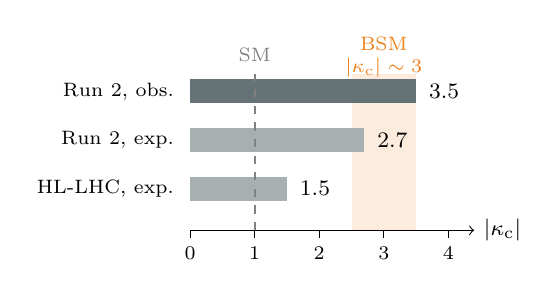
\begin{tikzpicture}[x=0.82cm,y=0.62cm,font=\footnotesize]
      \fill[accB!15] (2.5,0.4) rectangle (3.5,3.6);
      \node[accB,font=\scriptsize,align=center] at (3.0,3.95) {BSM\\$|\kc|\sim3$};
      \fill[accA!70] (0,3) rectangle (3.5,3.5);
      \fill[accA!40] (0,2) rectangle (2.7,2.5);
      \fill[accA!40] (0,1) rectangle (1.5,1.5);
      \node[anchor=west] at (3.55,3.25) {3.5};
      \node[anchor=west] at (2.75,2.25) {2.7};
      \node[anchor=west] at (1.55,1.25) {1.5};
      \node[anchor=east,align=right,font=\scriptsize] at (-0.1,3.25) {Run 2, obs.};
      \node[anchor=east,align=right,font=\scriptsize] at (-0.1,2.25) {Run 2, exp.};
      \node[anchor=east,align=right,font=\scriptsize] at (-0.1,1.25) {HL-LHC, exp.};
      \draw[thick,gray,dashed] (1,0.4) -- (1,3.6);
      \node[gray,font=\scriptsize] at (1,4.0) {SM};
      \draw[->] (0,0.4) -- (4.4,0.4) node[right] {$|\kc|$};
      \foreach \x in {0,1,2,3,4} \draw (\x,0.4) -- (\x,0.25) node[below,font=\scriptsize] {\x};
    \end{tikzpicture}\\[0.3ex]
    {\scriptsize Run 2: \ttH+VH (PRL 136 (2026) 011801); HL-LHC: ATLAS+CMS, 3\,ab$^{-1}$ each\par}\callnote{Every bar still includes $\kc=0$}\par
    \vspace{4pt}
    \begin{resultbox}[fontupper=\footnotesize]
      \kc\ at $\mathcal{O}(1)$: first sensitivity to whether the Higgs gives charm its mass
    \end{resultbox}
  \end{columns}
\end{frame}

% ===================================================================
\begin{frame}[t]{Summary}
  \up
  \begin{keybox}[fontupper=\small]
    The charm Yukawa is the most accessible 2\textsuperscript{nd}-generation quark coupling; CMS probes it in decay, in production and indirectly
  \end{keybox}
  \vspace{3pt}
  {\small
  \pill{Direct}\ \ \ttH(\Hcc) + VH(\Hcc): \textbf{$|\kc| < \obsexp{3.5}{2.7}$}, the most stringent direct constraint and the best expected sensitivity\par\vspace{4pt}
  \pill{Production}\ \ H+c: $|\kc|<\obsexp{47}{51}$, independent of the \Hcc\ decay\par\vspace{4pt}
  \pill{Indirect}\ \ Off-shell + on-shell H$\to4\ell$: $\kc\in[-3.3,2.8]$ with $|\kappa_V|\le1$ (about $\pm8$ without)\par\vspace{4pt}
  \pill{Next}\ \ All \kc\ results are Run 2; Run 3 starts with better taggers, higher trigger efficiency and a measured \ttbar+\ccbar\ background\par}
  \vspace{6pt}
  \begin{resultbox}[fontupper=\small]
    \textbf{Does the Higgs give charm its mass?} Today $|\kc|\lesssim3$--3.5, entering BSM-motivated territory;\\
    HL-LHC expected $|\kc|<1.5$: approaching, not yet reaching, sensitivity to $\kc=0$
  \end{resultbox}
  \vfill
  {\centering\color{accA}\large\bfseries Thank you!\par}
\end{frame}

% ===================================================================
\appendix
\begin{frame}[standout]
  Backup
\end{frame}

\pubref{\href{\pubHIG{HIG-21-008}}{PRL 131 (2023) 061801}}
\begin{frame}[t]{VH(\Hcc): event categories and sensitivity}
  \up
  \begin{columns}[T]
    \column{0.32\textwidth}
    \centering
    \includegraphics[width=\linewidth]{HIG-21-008_Figure_001.pdf}\\
    {\scriptsize ParticleNet merged-jet \Hcc\ tagging\par}
    \column{0.32\textwidth}
    \centering
    \includegraphics[width=\linewidth]{HIG-21-008_Figure_002-b.pdf}\\
    {\scriptsize Events vs.\ $\log_{10}(S/B)$\par}
    \column{0.32\textwidth}
    \centering
    \includegraphics[width=\linewidth]{HIG-21-008_Figure-aux_001.pdf}\\
    {\scriptsize $|\kc|$ scan (supplementary)\par}
  \end{columns}
  \vspace{4pt}
  \begin{keybox}[fontupper=\small]
    Best fit $\mu = 7.7^{+3.8}_{-3.5}$; merged $\mu=8.7^{+4.6}_{-4.0}$, resolved $\mu=-9.5\pm9.6$. $\sigma\mathcal{B}<0.94$ (0.50) pb.
    $\mu$ limits with CLs; \kc\ intervals from profile-likelihood scans.
  \end{keybox}
  \takeaway{The upward fluctuation comes from the merged-jet category}
\end{frame}

\pubref{\href{\pubHIG{HIG-21-008}}{PRL 131 (2023) 061801; strategy as in JHEP 03 (2020) 131}}
\begin{frame}[t]{VH(\Hcc): analysis details}
  \up
  \begin{columns}[T]
    \column{0.60\textwidth}
    {\scriptsize
    \pill{Topologies} Two, orthogonal: H candidate from a large-R ($R=1.5$) jet with $p_\mathrm{T}$ above (merged) or below (resolved) 300\,GeV; same lepton channels\par\vspace{3pt}
    \pill{Resolved} DeepJet CvsL/CvsB; the two highest-CvsL jets form the H candidate; leading-jet cuts at $\approx$40\% c efficiency ($\approx$4\% light, $\approx$16\% b mistag). c-jet energy regression, FSR-jet recovery and a 2L kinematic fit improve the $m(\mathrm{H_{cand}})$ resolution by up to 20\%. BDT per channel, fit to the BDT score\par\vspace{3pt}
    \pill{Merged} ParticleNet \ccbar\ tagger, 4--7$\times$ better rejection than DeepAK15; 3 working points ($\approx$58, 40, 16\% \ccbar\ efficiency) define 3 purity categories. ParticleNet mass regression: $\approx$50\% better mass resolution. BDTs decorrelated from $m(\mathrm{H_{cand}})$; fit to $m(\mathrm{H_{cand}})$\par\vspace{3pt}
    \pill{Backgrounds} V+jets and \ttbar\ normalised in dedicated control regions, following the 2016 analysis (V+jets split by jet flavour, free rate parameters)\par\vspace{3pt}
    \pill{VZ validation} Same analysis, resolved BDTs retrained with VZ as signal, merged unchanged. $\mu_\mathrm{VZ} = 1.01^{+0.23}_{-0.21}$; 4.4$\sigma$ merged, 3.1$\sigma$ resolved, 5.7$\sigma$ combined (exp.\ 4.7, 3.3, 5.9)\par}
    \column{0.37\textwidth}
    \centering
    \pill{Uncertainty breakdown}\par\vspace{2pt}
    \scriptsize
    \renewcommand{\arraystretch}{1.05}
    \begin{tabular}{lr}
      \toprule
      Source & $\Delta\mu/\Delta\mu_\mathrm{tot}$\\
      \midrule
      \rowcolor{accB!12}\textbf{Statistical} & \textbf{85\%}\\
      \quad Bkg.\ normalisations & 37\%\\
      Experimental & 48\%\\
      \quad Simulated sample sizes & 37\%\\
      \quad c-jet identification & 23\%\\
      \quad Jet energy scale, resolution & 15\%\\
      \quad Simulation modelling & 11\%\\
      \quad Luminosity & 6\%\\
      \quad Lepton identification & 4\%\\
      Theory & 22\%\\
      \quad Backgrounds & 17\%\\
      \quad Signal & 15\%\\
      \bottomrule
    \end{tabular}\\[0.4ex]
    {\scriptsize For $\hat\mu = 7.7^{+3.8}_{-3.5}$; simulation size driven by negative weights in NLO V+jets\par}
  \end{columns}
  \takeaway{Statistics-limited; the c-tagging and simulation-size systematics come next}
\end{frame}

\pubref{\href{\pubHIG{HIG-24-018}}{PRL 136 (2026) 011801}}
\begin{frame}[t]{\ttH(\Hcc): event yields}
  \up
  \begin{columns}[T]
    \column{0.62\textwidth}
    \centering
    \includegraphics[width=\linewidth]{HIG-24-018_Figure_002.pdf}\\
    {\scriptsize Event yields vs.\ $\log_{10}(S/B)$; the \ttH(\ccbar) panel shows the published best fit $\hat\mu = -1.6\pm4.5$\par}
    \column{0.36\textwidth}
    \centering
    \includegraphics[width=\linewidth]{HIG-24-018_Figure_003.pdf}\\
    {\scriptsize $\mu_{\ttH(\ccbar)}$ limits per channel (inner band 68\%)\par}
  \end{columns}
  \takeaway{\ttH(\ccbar) best fit $\hat\mu = -1.6\pm4.5$: compatible with zero and with the SM}
\end{frame}

\pubref{\href{\pubHIG{HIG-24-018}}{PRL 136 (2026) 011801}}
\begin{frame}[t]{\ttH(\Hcc): flavour tagging and by-products}
  \up
  \begin{columns}[T]
    \column{0.45\textwidth}
    \pill{Tagging}\par\vspace{2pt}
    {\small
    $\bullet$ Each jet gets ParticleNet scores; the (b+c vs.\ light, b vs.\ c) plane is split into 2D categories\\
    $\bullet$ ParT event classifier separates \ttH(\ccbar), \ttH(\bbbar), \ttZ, \ttbar+HF\par}
    \vspace{5pt}
    \pill{By-products}\par\vspace{2pt}
    {\small
    $\bullet$ \ttZ(Z$\to\ccbar$) as a standard candle: $\mu = 1.0\pm0.8$\\
    $\bullet$ \ttH(\Hbb) $\mu=0.91^{+0.26}_{-0.22}$, 4.4$\sigma$ (4.5 exp.)\par}
    \column{0.52\textwidth}
    \centering
    \includegraphics[height=5.5cm]{HIG-24-018_Figure_001.pdf}\\
    {\scriptsize b, c, light jets in the ParticleNet (b+c vs.\ light, b vs.\ c) plane and the 2D tagging categories\par}
  \end{columns}
\end{frame}

\pubref{\href{\pubHIG{HIG-24-018}}{PRL 136 (2026) 011801 (supplementary)}}
\begin{frame}[t]{\ttH(\Hcc): validation region and QCD rejection}
  \up
  \begin{columns}[T]
    \column{0.62\textwidth}
    \centering
    \includegraphics[width=\linewidth]{HIG-24-018_Figure_0B6.pdf}\\
    {\scriptsize Validation region $0.4<D_{\ttbar X}<0.6$, same SR/CR structure (CR-like $0.40$--$0.58$, SR-like $0.58$--$0.60$): good agreement\par}
    \vspace{2pt}\raggedright
    {\scriptsize
    $\bullet$ c-enriched regions need $\geq$2 c jets (\ttbar+c: $\geq$1); CR choice weights 100, 12, 4, 2, 1 on the \ttbar+light, +c, +$\geq$2c, +b, +$\geq$2b scores\\
    $\bullet$ \ttbar+b, +$\geq$2b from a dedicated 4FS \ttbar\bbbar\ sample\par}
    \column{0.36\textwidth}
    \centering
    \includegraphics[width=\linewidth]{HIG-24-018_Figure_0B3.pdf}\\
    {\scriptsize 0L only: $D_\mathrm{QCD}<10^{-4}$ (grey area rejected) suppresses QCD by nearly four orders of magnitude, to $<$1\% of \ttbar+jets; QCD simulation is used only to train the classifier\par}
  \end{columns}
\end{frame}

\pubref{\href{\pubHIG{HIG-24-018}}{PRL 136 (2026) 011801}}
\begin{frame}[t]{\ttH(\Hcc/\Hbb): (\kb, \kc) plane}
  \up
  \begin{columns}[c]
    \column{0.5\textwidth}
    \centering
    \includegraphics[width=0.9\linewidth]{HIG-24-018_Figure_004.pdf}\\
    {\scriptsize orange: observed, blue: expected; dashed 68\%, solid 95\% CL\par}
    \column{0.45\textwidth}
    {\small
    $\bullet$ Simultaneous \ttH(\Hbb) + \ttH(\Hcc) fit constrains both Yukawas\\[2pt]
    $\bullet$ Signal strengths: \ttH(\bbbar) $0.91^{+0.26}_{-0.22}$; \ttH(\ccbar) $-1.6\pm4.5$; \ttZ(\bbbar) $1.47^{+0.45}_{-0.41}$; \ttZ(\ccbar) $1.02^{+0.79}_{-0.84}$\par}
    \vspace{6pt}
    \begin{resultbox}
      $|\kc| < 4.2$ obs.\ with \kb\ fitted
    \end{resultbox}
  \end{columns}
\end{frame}

\pubref{\href{\pubHIG{HIG-24-009}}{JHEP 08 (2026) 051}}
\begin{frame}[t]{cH(H$\to$WW): post-fit distributions and per-period limits}
  \up
  \begin{columns}[T]
    \column{0.60\textwidth}
    \centering
    \includegraphics[height=5.0cm]{HIG-24-009_Figure_005.pdf}\\
    {\scriptsize 1-POI post-fit distributions of the BDT discriminants\par}
    \column{0.36\textwidth}
    \centering
    \includegraphics[width=\linewidth]{HIG-24-009_Figure_006.pdf}\\
    {\scriptsize $\mu_\mathrm{cH}$ limits per data-taking period, 1 and 2 POI\par}
  \end{columns}
  \takeaway{Best fit (1 POI): $\mu_\mathrm{cH} = 390^{+380}_{-270}$, within 1.5$\sigma$ of the SM; statistics-limited}
\end{frame}

\pubref{\href{\pubHIG{HIG-24-009}}{JHEP 08 (2026) 051}}
\begin{frame}[t]{cH(H$\to$WW): floating the H+c background}
  \up
  \begin{columns}[c]
    \column{0.45\textwidth}
    {\small
    $\bullet$ \pill{1 POI} only $\mu_\mathrm{cH}$ floats; the \kc-independent H+c background (from ggH etc.) is fixed to its SM prediction\\[3pt]
    $\bullet$ \pill{2 POI} H+c background also floats; correlation with cH: $-87\%$\\[3pt]
    $\bullet$ 2-POI limit: $\mu_\mathrm{cH} < \obsexp{1804}{1097}$\\[3pt]
    $\bullet$ The combination with $\gamma\gamma$ uses the 1-POI fit\par}
    \column{0.50\textwidth}
    \centering
    \includegraphics[width=0.9\linewidth]{HIG-24-009_Figure_007.pdf}\\
    {\scriptsize WW: $\mu_\mathrm{cH}$ vs.\ $\mu_{\mathrm{H+c\,bkg}}$\par}
  \end{columns}
  \takeaway{Floating the H+c background weakens the WW limit from 1065 to 1804}
\end{frame}

\begin{frame}[t]{Indirect: Higgs \texorpdfstring{$p_\mathrm{T}$}{pT} spectrum and on-shell H\texorpdfstring{$\to4\ell$}{->4l}}
  \up
  \begin{columns}[T]
    \column{0.50\textwidth}
    \centering
    \includegraphics[height=5.3cm,trim=0 0 205 0,clip]{HIG-23-013_Figure_006.pdf}\\
    {\scriptsize JHEP 04 (2026) 093: (\kb, \kc) from the Run 2 $p_\mathrm{T}^\mathrm{H}$ combination ($\gamma\gamma$, ZZ, resolved $\tau\tau$), $\mathcal{B}$ coupling-dependent; 2D contours only\par}
    \column{0.46\textwidth}
    \centering
    \includegraphics[height=5.3cm,trim=180 0 0 176,clip]{HIG-23-011_Figure_009.pdf}\\
    {\scriptsize PRD 112 (2025) 112001 ($\gamma$H + on-shell H$\to4\ell$): \kc\ scan; solid obs., dashed exp.\par}
  \end{columns}
\end{frame}

\pubref{\href{\pubHIG{SMP-22-012}}{PLB 865 (2025) 139462, CMS-SMP-22-012}}
\begin{frame}[t]{Rare exclusive decays: H$\to$J/$\psi\gamma$, $\psi$(2S)$\gamma$}
  \up
  \begin{columns}[c]
    \column{0.48\textwidth}
    {\small
    $\bullet$ Direct ($\propto\kc$) and indirect (H$\to\gamma\gamma^*\to\gamma\,$J/$\psi$) amplitudes interfere $\Rightarrow$ sign sensitivity\\[2pt]
    $\bullet$ 123\fbinv: $\mathcal{B}(\mathrm{H}\to\mathrm{J}/\psi\gamma) < 2.6\times10^{-4}$, $\mathcal{B}(\mathrm{H}\to\psi(2\mathrm{S})\gamma) < 9.9\times10^{-4}$\par}
    \vspace{6pt}
    \begin{resultbox}[fontupper=\footnotesize]
      $\kc/\kappa_\gamma\in(-157,199)$; with $\kappa_\gamma=1$: $\kc\in(-166,208)$\\
      {\color{gray}exp.\ $(-128,169)$, 95\% CL}
    \end{resultbox}
    \column{0.45\textwidth}
    \centering
    \includegraphics[width=0.9\linewidth]{SMP-22-012_Figure_005.pdf}\\
    {\scriptsize 95\% CL upper limits on $\mathcal{B}$(Z, H$\to\psi(n\mathrm{S})\gamma$), obs.\ and exp.\par}
  \end{columns}
\end{frame}

\pubref{\href{\pubHIG{HIG-19-006}}{JHEP 01 (2021) 148, CMS-HIG-19-006}}
\begin{frame}[t]{H$\to\mu\mu$: evidence for a 2\textsuperscript{nd}-generation Yukawa}
  \up
  \begin{columns}[T]
    \column{0.36\textwidth}
    {\small
    $\bullet$ 137\fbinv, four categories: ggH, VBF, VH, \ttH\\[2pt]
    $\bullet$ Excess of \textbf{3.0$\sigma$} (2.5$\sigma$ exp.): first evidence for H decays to 2\textsuperscript{nd}-generation fermions\\[2pt]
    $\bullet$ $\mu = 1.19^{+0.40}_{-0.39}\,(\mathrm{stat})^{+0.15}_{-0.14}\,(\mathrm{syst})$\\[2pt]
    $\bullet$ $\kappa_\mu = 1.07$; 95\% CL: $0.59<\kappa_\mu<1.50$ {\scriptsize(6 free $\kappa$, SM total width)}\\[2pt]
    {\scriptsize Rare decays incl.\ $\mu\mu$: L.~D'Eramo's plenary (Wed)}\par}
    \column{0.30\textwidth}
    \centering
    \includegraphics[width=\linewidth]{HIG-19-006_Figure_011-a.pdf}\\
    {\scriptsize $\hat\mu$ per production category and combined\par}
    \column{0.30\textwidth}
    \centering
    \includegraphics[width=\linewidth]{HIG-19-006_Figure_014-a.pdf}\\
    {\scriptsize $-2\Delta\ln L$ vs.\ $\kappa_\mu$\par}
  \end{columns}
  \takeaway{The muon Yukawa is SM-like within about 20\% (68\% CL); charm is the next 2\textsuperscript{nd}-generation test}
\end{frame}

\pubref{\href{\pubHIG{BTV-25-002}}{arXiv:2608.18331, CMS-BTV-25-002}}
\begin{frame}[t]{Run 3 HLT flavour tagging}
  \up
  \begin{columns}[T]
    \column{0.48\textwidth}
    \centering
    \includegraphics[height=5.5cm,trim=0 0 197 0,clip]{BTV-25-002_Figure_005.pdf}\\
    {\scriptsize Simulation, jet $p_\mathrm{T}$ 30--100\,GeV: light (solid) and b (dashed) misidentification vs.\ c-jet efficiency, online vs.\ offline taggers\par}
    \column{0.48\textwidth}
    \centering
    \includegraphics[height=5.5cm,trim=0 0 199 0,clip]{BTV-25-002_Figure_023.pdf}\\
    {\scriptsize Simulation: VBF H$\to\ccbar$ trigger efficiency vs.\ offline ParticleNet c score, Run 3 VBF H$\to\ccbar$ vs.\ Run 2 VBF H$\to\bbbar$ trigger\par}
  \end{columns}
\end{frame}

\begin{frame}[t]{Likely questions}
  \up
  \footnotesize
  \begin{itemize}\setlength\itemsep{1pt}
    \item \textbf{How large is the VH excess?} Best fit $\mu_\mathrm{VH} = 7.7^{+3.8}_{-3.5}$, about 1.9$\sigma$ above $\mu=1$ (estimated from the quoted uncertainty; the paper calls it a small upward fluctuation). This is why VH alone excludes $|\kc|<1.1$ and why \ttH\ alone (3.0) beats the combination (3.5) on observed
    \item \textbf{What limits the direct searches?} Statistics first. \ttH(\ccbar): statistical 74\% of the total uncertainty, then \ttbar+c and \ttbar+light modelling ($\approx$32\%, $\approx$29\%). VH(\ccbar): simulation sample size ($\approx$37\%), c-tagging efficiency ($\approx$23\%), theory ($\approx$22\%)
    \item \textbf{And ATLAS?} VBF + VH(\Hcc) (arXiv:2511.21911): $|\kc| < 4.7$ (3.9 exp.), same assumptions as CMS (other couplings SM, no BSM decays); its VBF part includes 51.5\fbinv\ of Run 3 data
    \item \textbf{Why is cH an order of magnitude weaker than \Hcc?} cH $\sigma\mathcal{B}$ is tiny ($\approx$0.2\,fb in $\gamma\gamma$) and ggH produces the same H+c final state independently of \kc; in \Hcc, \kc\ changes the branching fraction of Higgs bosons from much larger production modes (VH, \ttH)
    \item \textbf{Why is cH($\gamma\gamma$) obs.\ (38) much better than exp.\ (73)?} The best fit is negative, $\hat\mu_\mathrm{cH} = -230^{+170}_{-251}$
    \item \textbf{Why no \kc\ from boosted \Hcc?} The paper quotes only $\mu$; the result is ggH-dominated
    \item \textbf{How much of the Run 3 trigger gain is the tagger?} Part of it is rate budget: 10\,Hz in 2018 vs.\ 60, 115, 170\,Hz in 2022, 2023, 2024
    \item \textbf{Are the H$\to4\ell$ intervals sign-sensitive?} Not really: the small asymmetry comes from charm-loop interference in ggH and H$\to$gg; the constraint is essentially on $\kc^2$
  \end{itemize}
\end{frame}

\begin{frame}[t]{References}
  \up
  \scriptsize
  \begin{itemize}\setlength\itemsep{0pt}
    \item VH(\Hcc): CMS, PRL 131 (2023) 061801, arXiv:2205.05550 (HIG-21-008)
    \item \ttH(\Hcc) + VH combination: CMS, PRL 136 (2026) 011801, arXiv:2509.22535 (HIG-24-018)
    \item VH(\Hcc) with 2016 data (analysis strategy): CMS, JHEP 03 (2020) 131, arXiv:1912.01662 (HIG-18-031)
    \item Boosted \Hcc: CMS, PRL 131 (2023) 041801, arXiv:2211.14181 (HIG-21-012)
    \item cH(H$\to\gamma\gamma$): CMS, JHEP 11 (2025) 060, arXiv:2503.08797 (HIG-23-010)
    \item cH(H$\to$WW) and combination: CMS, JHEP 08 (2026) 051, arXiv:2508.14988 (HIG-24-009)
    \item Differential combination Run 2: CMS, JHEP 04 (2026) 093, arXiv:2504.13081 (HIG-23-013)
    \item $\gamma$H + H$\to4\ell$ light Yukawas: CMS, PRD 112 (2025) 112001, arXiv:2502.05665 (HIG-23-011)
    \item Off-shell + on-shell H$\to4\ell$: CMS, arXiv:2607.23352, submitted to PRD (HIG-25-003)
    \item H$\to$J/$\psi\gamma$: CMS, PLB 865 (2025) 139462, arXiv:2411.15000 (SMP-22-012)
    \item H$\to\mu\mu$: CMS, JHEP 01 (2021) 148, arXiv:2009.04363 (HIG-19-006)
    \item Jet flavour tagging in Run 3: CMS-DP-2025-081; DeepJet: E.~Bols et al., JINST 15 (2020) P12012
    \item HLT flavour tagging: CMS, arXiv:2608.18331 (BTV-25-002)
    \item \ttbar+b/c cross sections: CMS-PAS-TOP-26-003
    \item ATLAS VBF + VH(\Hcc): ATLAS, arXiv:2511.21911
    \item HL-LHC: ATLAS and CMS, arXiv:2504.00672 (HIG-25-002)
    \item Higgs combination: CMS, Rep. Prog. Phys. 89 (2026) 087801, arXiv:2602.18611 (HIG-21-018)
    \item Spontaneous flavour violation: arXiv:2410.05236
    \item HL-LHC Yellow Report: M.~Cepeda et al., CERN Yellow Rep.\ Monogr.\ 7 (2019) 221, arXiv:1902.00134
  \end{itemize}
\end{frame}

\end{document}
